% Template for PLoS
% Version 3.6 Aug 2022
%
% % % % % % % % % % % % % % % % % % % % % %
%
% -- IMPORTANT NOTE
%
% This template contains comments intended 
% to minimize problems and delays during our production 
% process. Please follow the template instructions
% whenever possible.
%
% % % % % % % % % % % % % % % % % % % % % % % 
%
% Once your paper is accepted for publication, 
% PLEASE REMOVE ALL TRACKED CHANGES in this file 
% and leave only the final text of your manuscript. 
% PLOS recommends the use of latexdiff to track changes during review, as this will help to maintain a clean tex file.
% Visit https://www.ctan.org/pkg/latexdiff?lang=en for info or contact us at latex@plos.org.
%
%
% There are no restrictions on package use within the LaTeX files except that no packages listed in the template may be deleted.
%
% Please do not include colors or graphics in the text.
%
% The manuscript LaTeX source should be contained within a single file (do not use \input, \externaldocument, or similar commands).
%
% % % % % % % % % % % % % % % % % % % % % % %
%
% -- FIGURES AND TABLES
%
% Please include tables/figure captions directly after the paragraph where they are first cited in the text.
%
% DO NOT INCLUDE GRAPHICS IN YOUR MANUSCRIPT
% - Figures should be uploaded separately from your manuscript file. 
% - Figures generated using LaTeX should be extracted and removed from the PDF before submission. 
% - Figures containing multiple panels/subfigures must be combined into one image file before submission.
% For figure citations, please use "Fig" instead of "Figure".
% See http://journals.plos.org/plosone/s/figures for PLOS figure guidelines.
%
% Tables should be cell-based and may not contain:
% - spacing/line breaks within cells to alter layout or alignment
% - do not nest tabular environments (no tabular environments within tabular environments)
% - no graphics or colored text (cell background color/shading OK)
% See http://journals.plos.org/plosone/s/tables for table guidelines.
%
% For tables that exceed the width of the text column, use the adjustwidth environment as illustrated in the example table in text below.
%
% % % % % % % % % % % % % % % % % % % % % % % %
%
% -- EQUATIONS, MATH SYMBOLS, SUBSCRIPTS, AND SUPERSCRIPTS
%
% IMPORTANT
% Below are a few tips to help format your equations and other special characters according to our specifications. For more tips to help reduce the possibility of formatting errors during conversion, please see our LaTeX guidelines at http://journals.plos.org/plosone/s/latex
%
% For inline equations, please be sure to include all portions of an equation in the math environment. For example, x$^2$ is incorrect; this should be formatted as $x^2$ (or $\mathrm{x}^2$ if the romanized font is desired).
%
% Do not include text that is not math in the math environment. For example, CO2 should be written as CO\textsubscript{2} instead of CO$_2$.
%
% Please add line breaks to long display equations when possible in order to fit size of the column. 
%
% For inline equations, please do not include punctuation (commas, etc) within the math environment unless this is part of the equation.
%
% When adding superscript or subscripts outside of brackets/braces, please group using {}. For example, change "[U(D,E,\gamma)]^2" to "{[U(D,E,\gamma)]}^2". 
%
% Do not use \cal for caligraphic font. Instead, use \mathcal{}
%
% % % % % % % % % % % % % % % % % % % % % % % % 
%
% Please contact latex@plos.org with any questions.
%
% % % % % % % % % % % % % % % % % % % % % % % %

\documentclass[10pt,letterpaper]{article}
\usepackage[top=0.85in,left=2.75in,footskip=0.75in]{geometry}

\usepackage[utf8]{inputenc}

% amsmath and amssymb packages, useful for mathematical formulas and symbols
\usepackage{amsmath,amssymb}

% Use adjustwidth environment to exceed column width (see example table in text)
\usepackage{changepage}

% textcomp package and marvosym package for additional characters
\usepackage{textcomp,marvosym}

% cite package, to clean up citations in the main text. Do not remove.
\usepackage{cite}

% Use nameref to cite supporting information files (see Supporting Information section for more info)
\usepackage{nameref,hyperref}

% line numbers
\usepackage[right]{lineno}

% ligatures disabled
\usepackage[nopatch=eqnum]{microtype}
\DisableLigatures[f]{encoding = *, family = * }

% color can be used to apply background shading to table cells only
\usepackage[table]{xcolor}

% array package and thick rules for tables
\usepackage{array}

% create "+" rule type for thick vertical lines
\newcolumntype{+}{!{\vrule width 2pt}}

% create \thickcline for thick horizontal lines of variable length
\newlength\savedwidth
\newcommand\thickcline[1]{%
 \noalign{\global\savedwidth\arrayrulewidth\global\arrayrulewidth 2pt}%
 \cline{#1}%
 \noalign{\vskip\arrayrulewidth}%
 \noalign{\global\arrayrulewidth\savedwidth}%
}

% \thickhline command for thick horizontal lines that span the table
\newcommand\thickhline{\noalign{\global\savedwidth\arrayrulewidth\global\arrayrulewidth 2pt}%
\hline
\noalign{\global\arrayrulewidth\savedwidth}}


% Remove comment for double spacing
%\usepackage{setspace} 
%\doublespacing

% Text layout
\raggedright
\setlength{\parindent}{0.5cm}
\textwidth 5.25in 
\textheight 8.75in

% Bold the 'Figure #' in the caption and separate it from the title/caption with a period
% Captions will be left justified
\usepackage[aboveskip=1pt,labelfont=bf,labelsep=period,justification=raggedright,singlelinecheck=off]{caption}
\renewcommand{\figurename}{Fig}

% Use the PLoS provided BiBTeX style
\bibliographystyle{plos2015}

% Remove brackets from numbering in List of References
\makeatletter
\renewcommand{\@biblabel}[1]{\quad#1.}
\makeatother



% Header and Footer with logo
\usepackage{lastpage,fancyhdr,graphicx}
\usepackage{epstopdf}
%\pagestyle{myheadings}
\pagestyle{fancy}
\fancyhf{}
%\setlength{\headheight}{27.023pt}
%\lhead{\includegraphics[width=2.0in]{PLOS-submission.eps}}
\rfoot{\thepage/\pageref{LastPage}}
\renewcommand{\headrulewidth}{0pt}
\renewcommand{\footrule}{\hrule height 2pt \vspace{2mm}}
\fancyheadoffset[L]{2.25in}
\fancyfootoffset[L]{2.25in}
\lfoot{\today}

%% Include all macros below

\newcommand{\Pro}[1]{P\left(#1\right)} 
\newcommand{\ProT}[1]{P_\theta\left(#1\right)} 
\newcommand{\Ex}[1]{\textbf{E}\left[#1\right]} 
\newcommand{\Var}[1]{\mathrm{Var}\left(#1\right)} 

%% END MACROS SECTION

\usepackage{booktabs}

\begin{document}
\vspace*{0.2in}

% Title must be 250 characters or less.
\begin{flushleft}
{\Large
\textbf\newline{Tractable time tree distributions} % Please use "sentence case" for title and headings (capitalize only the first word in a title (or heading), the first word in a subtitle (or subheading), and any proper nouns).
}
\newline
% Insert author names, affiliations and corresponding author email (do not include titles, positions, or degrees).
\\
Tobia Ochsner\textsuperscript{1, 2}*,
Jonathan Klawitter\textsuperscript{1},
Alexei J. Drummond\textsuperscript{1}*,
\\
\bigskip
\textbf{1} University of Auckland, Auckland, Aotearoa/New Zealand
\\
\textbf{2} ETH Zurich, Basel, Switzerland
\\
\bigskip

% Use the asterisk to denote corresponding authorship and provide email address in note below.
* a.drummond@auckland.ac.nz

\end{flushleft}
% Please keep the abstract below 300 words
\section*{Abstract}
In Bayesian phylogenetics, Markov Chain Monte Carlo (MCMC) methods generate samples of time trees to capture the posterior distribution of the phylogenetic tree. We explore novel approaches to fit distributions on these time trees samples. In particular, we extend the family of Conditional Clade Distributions (CCD) to model the tree topology and branch lengths simultaneously. Our distributions are designed to capture both central tendencies and dependencies within this high-dimensional and non-Euclidean space. They facilitate a straightforward reconstruction of a summary tree and manage to capture the tails of the time tree distribution. This property extends their utility beyond the robust reconstruction of a single summary tree, enabling more sophisticated downstream analyses like exploring credible sets or evaluating alternative evolutionary hypotheses.


% Please keep the Author Summary between 150 and 200 words
% Use first person. PLOS ONE authors please skip this step. 
% Author Summary not valid for PLOS ONE submissions.  
\section*{Author summary}


\linenumbers

% Use "Eq" instead of "Equation" for equation citations.
\section*{Introduction}

Markov Chain Monte Carlo (MCMC) methods have become a cornerstone of Bayesian phylogenetics. Given a set of aligned molecular sequences and an evolutionary model (consisting of a tree model, a molecular clock model, a substitution model, and prior distributions on parameters), MCMC algorithms like Beast 2 \cite{beast2} or MrBayes \cite{mrbayes} generate a set of phylogenetic trees sampled from the posterior distribution. This posterior sample usually consists of thousands of trees and contains a wealth of information about the evolutionary relationships encoded in the provided sequences.

For simple continuous or indicator parameters of the phylogenetic model (like substitution or clock rates), analyzing the marginal distributions of the posterior sample is relatively straightforward. Tools like Tracer \cite{tracer} provide readily available summaries and visualizations of these marginal distributions.

The space of phylogenetic trees presents a significantly greater challenge. The sheer number of possible rooted trees explodes super-exponentially with increasing taxa, making it highly unlikely that the MCMC samples contain the true tree topology \cite{ccd}. The \emph{curse of dimensionality} \cite{curse} diminishes the effectiveness of common sample-based statistical methods, particularly distance-based approaches. We demonstrate in the Supplementary Information that MCMC samples can exhibit strikingly similar pairwise distances, contradicting the expectation that regions of higher probability density should yield samples with closer proximity. Furthermore, the space of possible node times is non-Euclidean, as the times are inherently constrained by the topology \cite{wald,tauspace,tropical,bhv}. These challenges make it difficult to directly analyze the posterior sample of trees and branch lengths. One strategy to extract meaningful information from the sample involves dedicated post-processing techniques. The raw sample is distilled into representations that enable a more meaningful analysis and interpretation.

A common approach is to infer a point estimate, a single "best" tree that summarizes the posterior sample \cite{treesinforest}. Several heuristics have been developed for this purpose, including DensiTree visualizations \cite{densitree}, Maximum Clade Credibility (MCC) trees, Hipster \cite{hipstr}, and the Maximum A Posteriori tree based on Conditional Clade Distributions (CCD) \cite{ccd,ccdlarget}. These methods often focusing primarily on recovering a likely tree topology. The determination of branch lengths is treated as an afterthought, potentially overlooking important information about evolutionary timescales.

Another class of algorithms considers both tree topology and branch lengths simultaneously by embedding trees in a defined metric space. Examples include the Billera-Holmes-Vogtmann (BHV) space \cite{bhv}, the Wald space \cite{wald}, the $t$ and $\tau$ space \cite{tauspace}, the palm tree space \cite{tropical}, the RNNI space \cite{rnnispace}, and the recently developed Wald space \cite{wald}. Within these spaces, a natural approach to obtaining a point estimate is to calculate the Fréchet mean of the posterior tree sample \cite{frechetmeanvar}. However, these spaces often suffer from limitations such as the "sticky mean" problem (where the mean tree is almost independent of the actual tree samples) \cite{sticky}, high computational complexity associated with distance calculations, and the inherent difficulties of performing statistical inference in complex geometric spaces \cite{riemanngaussian}.

While obtaining a point estimate from the posterior sample is crucial, it is important to recognize that the MCMC sample embodies information about the entire posterior distribution. Tractable tree distributions \cite{ccd} aim to capture the posterior distribution using a well-defined approximate distribution. This provides an elegant framework for testing alternative evolutionary hypotheses, determining whether a specific tree falls within a credible set, calculating statistics like information content \cite{informationcontent}, and analyzing dependencies between different parts of the tree (e.g., relationships between branch lengths and topological features). Existing methods that estimate distributions on the posterior sample for rooted trees focus on modeling tree topologies \cite{ccd,ccdlarget}, ignoring time information entirely. The family of Bayesian subsplit networks \cite{subsplit} has been extended to model branch lengths in multiple ways \cite{subsplitnf,subsplitbranchlengths}. However, Bayesian subsplit methods focus on direct variational inference, rather than posterior sample summarization.

This paper addresses the challenge of inferring tractable distributions on time trees, encompassing both topology and branch lengths. We compare different methods and tree embeddings, and demonstrate that the described methods exhibit significant differences in terms of capturing central tendencies and the tails of the distribution. Finally, we introduce a software package that enables researchers to fit and analyze these distributions, facilitating more nuanced insight into phylogenetic uncertainty. This tool allows for a more complete utilization of the information contained within the posterior tree sample, moving beyond simple point estimates.

\section*{Materials and methods}

In this section, we introduce the concept of tractable tree distributions on time trees and discuss desirable properties of such distributions. We then introduce a family of distributions satisfying these properties and show how to estimate the parameters based on a tree sample. Furthermore, we describe how these distributions lead to a point estimator. Finally, we outline the procedure used to assess and compare the distributions on both synthetic and real datasets.

\subsection*{Tractable tree distributions}

Berling et al. \cite{ccd} introduced \emph{tractable tree distributions} as a set of properties of a distribution on tree topologies. A distribution is tractable if a range of operations can be performed efficiently in practice. We apply the same concept to distributions on \emph{time trees}.

Tractable time tree distributions are used as a tool to analyze a posterior tree sample. Therefore, we should be able to efficiently infer its parameters based on that tree sample. In order to compare different tree hypotheses, we need to evaluate the probability of any time tree under the model. Another important operation is sampling, as it enables to test if a tree is in the 95\% credible set and to inspect the dependencies of different node heights. Lastly, a tractable time tree distribution should provide us with a \emph{summary tree}, for instance by retrieving the highest-probability or expected tree.

\subsection*{Mathematical framework}

A \emph{time tree} $(T, \{H_v\}_{v \in V})$ for a set of taxa $X$ and root $R$ consists of a tree $T = (V, E)$ and a set of random variables $\{H_v\}_{v \in V} \in \mathbb{R}^+$ denoting the vertex heights. The following properties have to be satisfied:

\begin{enumerate}
	\item $(V, E)$ describe a fully connected tree.
	\item The root $R \in V$ has degree $2$. The taxa $X \subset V$ have degree $1$. All other vertices are \emph{internal} vertices and have degree $3$.
	\item We only consider contemporary sampling of the taxa: $H_x = 0$ for all taxa $x$.
	\item Each edge $e$ in $E$ consists of a parent $p$ and child $c$ such that the parent is closer to the root. The heights must describe a valid tree and evolution runs backward in time: $H_c < H_p$ for all edges $(p, c)$ in $E$.
\end{enumerate}

The probability of a time tree can be factorized into the probability of its topology $T$ and the probability of the vertex heights $\{H_v\}$ given the topology:

$$
\Pro{(T, \{H_v\})} = \Pro{T} \Pro{\{H_v\} | T}.
$$

To model $\Pro{T}$, we use the conditional clade distributions \emph{CCD0} and \emph{CCD1} \cite{ccd,ccdlarget}. They already exhibit the desired properties and have shown to work well in practice \cite{ccd,ccd0expansion,hipstr}. Thus, we focus on modelling the conditional probability $\Pro{\{H_v\} | T}$. It is crucial to note that we do not restrict ourselves to a single topology $T$---we simply model $\Pro{\{H_v\} | T}$ as a function of the topology $T$.

\subsection*{Clade parameterisation}

There are two main challenges when designing a distribution on the heights:

First, $P\left(\{H_v\} | T\right)$ is a function of the topology $T$. However, we cannot assume that every possible topology is found in the MCMC sample. Hence, $P\left(\{H_v\} | T\right)$ needs to be defined even for unknown topologies. Moreover, as the number of possible topologies can be extremly large, we have to share parameters amongst different topologies. In order to overcome this challenge, we employ the same strategy as the CCD0 model \cite{ccd}: instead of having random variables corresponding to vertices of a topology, they correspond to clades:

$$
\Pro{\{H_v\} | T} = \Pro{\{H_c\}_{c \in C(T)} | T},
$$

where $C(T)$ is the set of clades in topology $T$. A clade is a subset of taxa that share a common ancestor. While every vertex corresponds to exactly one clade, modeling random variables on a clade-level allows to share parameters amongst different topologies that have common clades. We call a clade \emph{non-trivial} if it is neither a singleton nor the root clade. In the following, we exclude the singleton clades corresponding to the taxa from $C(T)$. $H_c$ equals $0$ for all singleton clades and does not need to be modelled. 

Another difficulty is the fact that every topology enforces a different set of constraints on the heights. We expect $P\left(\{H_c\} | T\right)$ to vanish for heights invalid under the topology. We solve this by introducing the concept of a \emph{clade embedding}. Given a topology $T$, a clade embedding $f_T$ induces a bijection from the heights into another set of random variables in the \emph{embedding space}:

$$
f_T: \{H_c\}_{c \in C(T)} \mapsto \{Z_c\}_{c \in C(T)}.
$$

The embedding can be chosen such that the $Z_c$ have nice constraints independent of the topology (for instance, $Z_c \in \mathbb{R}$ or $Z_c \in [0, 1]$). Equipped with an embedding, we can define a probability distribution on $\{Z_c\}$ as well as the corresponding pulled-back probability distribution on $\{H_c\}$:

$$
P\left(\{H_c\} | T\right) = P\left(\{Z_c\} | T\right) \left| \det{\left(J_{f_t^{-1}}(\{Z_c\})\right)} \right|,
$$

where $J_{f_t^{-1}}(\{Z_c\})$ is the Jacobian of the inverse of the embedding.

In order to get the probability of a set of heights under a topology, we first transform the set of heights into the embedding space. Then, we can use the pulled-back probability distribution to calculate the probability. If we want to sample from the distribution, we can sample from the embedding space and transform the samples back into the original height space.

In the following sections, we introduce three different clade embeddings as well as different strategies for assigning probabilities in the embedding space. Our general approach is to find the best approximation of the marginal time tree posterior distribution of the MCMC model. Thus, biological interpretation of the designed distributions is not a primary goal. Instead, we focus on a wide range of embeddings and distributions that fulfill the properties of tractable time tree distributions and then compare their fit with the MCMC posterior distribution of a variety of real and simulated datasets.

\subsection*{Last divergence embedding}

Under the birth death model, internal branch lengths are assumed to be independent realizations of a stochastic evolutionary process. In contrast, pendant branch lengths are primarily influenced by the time of sampling. We propose to model internal branch lengths using independent distributions, while separatly accounting for the time between sampling and the last divergence event. This approach aligns with theoretical findings suggesting that internal and pendant branch lengths follow notably different distributions \cite{birthdeathdistribution,birthdeathdistributionstadler}.

Specifically, we consider the branch length leading to a vertex $v$ corresponding to a non-trivial clade $c$:

$$
Z_c = H_{p_v} - H_v.
$$

Furthermore, we consider the time between the present and the last divergence event and assign it to the random variable corresponding to the root clade $X$:

$$
Z_X = \min_{x \in X}{H_x}.
$$

This embedding allows to choose arbitrary positive $Z_c$ while always producing a valid tree. Thus, we propose to use either independent lognormal, independent gamma distributions, or independent Weibull distributions:

$$
P(\{Z_c\}_{c \in C(T)}) = \begin{cases}
	\prod_{c \in C(T)}{LogNormal(Z_c; \mu_c, \sigma_c)}, \\
	\prod_{c \in C(T)}{Gamma(Z_c; \alpha_c, \beta_c)}, \\
	\prod_{c \in C(T)}{Weibull(Z_c; k_c, \lambda_c)}.
\end{cases}
$$

Different models for divergence suggest different distributions on the branch lengths \cite{venditti2010phylogenies}. For instance, a constant rate of divergence will result in an exponential distribution, which is a special case of the gamma distribution. If the rate of divergence changes with the amount of time since the last divergence, the resulting distribution is a Weibull distribution.

\subsection*{Oldest child embedding}

We introduce an alternative embedding that directly utilizes absolute branch lengths. For a clade $c$ corresponding to vertex $v$, we define $Z_c$ as the branch length leading to the older child of $v$.

$$
Z_c = H_v - \max{\left(H_{a_v}, H_{b_v}\right)},
$$

where $a_v$ and $b_v$ represent the two child vertices of $v$. This parameterisation ensures that any set of positive $Z_c$, given a topology, results in a valid contemporary sampled time tree. To assign probabilities to these branch lengths, we consider same three probabilistic models:

$$
P(\{Z_c\}_{c \in C(T)}) = \begin{cases}
	\prod_{c \in C(T)}{LogNormal(Z_c; \mu_c, \sigma_c)}, \\
	\prod_{c \in C(T)}{Gamma(Z_c; \alpha_c, \beta_c)}, \\
	\prod_{c \in C(T)}{Weibull(Z_c; k_c, \lambda_c)}.
\end{cases}
$$

\subsection*{Height ratio embedding}

Inspired by TreeFlow \cite{treeflow}, we introduce the height ratio embedding to capture the relative temporal structure of the vertices in time trees. For any non-trivial clade $c$ correspoding to vertex $v$, we define $Z_c$ as the ratio of the height of $v$ to the height of its parent vertex $p_v$.

$$
Z_c = \frac{H_v}{H_{p_v}}.
$$

In addition to the relative positions of the vertices, we model the overall height of the time tree using the random variable corresponding to the root clade $X$:

$$
Z_X = H_R.
$$

Consequently, $Z_X$ takes values in $\mathbb{R}^+$. For any non-trivial clade $c$, $Z_c$ is constrained to the interval $[0, 1]$. The primary advantage of the height ratio embedding lies in its ability to mitigate the effects of dependencies introduced by contemporary sampling.

We model the ratios and the tree height independently. For the height ratios, we consider the following probability distributions:

$$
P(\{Z_c\}_{c \in C(T) \setminus X}) = \begin{cases}
	\prod_{c \in C(T) \setminus X}{Beta(Z_c; \alpha_c, \beta_c)}, \\
	\prod_{c \in C(T) \setminus X}{LogitNormal(Z_c; \mu_c, \sigma_c)}, \\
	TreeDirichlet(Z_c; \{\alpha_c\}_{c \in C(T) \setminus X}).
\end{cases}
$$

The $TreeDirichlet$ distribution is a generalized Dirichlet distribution, parameterized by a single parameter for each non-trivial clade. It is a special case of the independent beta distributions, defined such that the marginal distribution of any path from the root vertex to a leaf follows a Dirichlet distribution. A formal definition is provided in the supporting information.

For the overall tree height, we employ a lognormal distribution:

$$
P(Z_X) = \text{Lognormal}(Z_X; \mu_X, \sigma_X).
$$

\subsection*{Operations on tractable time tree distributions}

We use the maximum likelihood estimator to estimate the parameters for each embedding and the corresponding distributions. The stated independence assumptions significantly simplify this process, reducing it to the maximum likelihood estimation of basic univariate continuous distributions. For the lognormal and logitnormal distribution, the maximum likelihood estimators exhibit well-known closed form solutions. For the gamma, beta and weibull distributions, we apply Newton's method as implemented in the julia package \emph{Distributions.jl} \cite{Distributions.jl}. The maximum likelihood estimator for the TreeDirichlet distribution is more involved and is detailed in the supporting information.

In order to calculate the probability for a given time tree, we first transform the set of heights into the embedding space. Then, we can use the pulled-back probability distribution to calculate the probability.

Sampling from the distribution is achieved by drawing samples from the embedding space and mapping them back to the original height space using the inverse transformation. To assess if a given time tree is within the 95 \% credible set, we can generate a large number of samples from the fitted distribution. If the model probability of the given tree ranks within the top 95 \% of the sampled tree probabilities, it is in the credible set."

\subsection*{Validation}

To evaluate the quality of our proposed tractable time tree distributions, we use two complementary methods: model comparison and goodness-of-fit (GoF) testing.

Given a posterior set of time trees, we calculate the Akaike Information Criterion (AIC) to compare the relative performance of our distributions on a given set of time trees. AIC balances model likelihood with parameter count, providing a ranking of models. However, it does not determine if any model accurately reflects the posterior distribution.

We perform a goodness-of-fit test to assess how well our tractable tree distributions capture the true distribution. We frame this as a two-sample hypothesis test, where we compare the MCMC time trees with a set of time trees sampled from our approximate distribution. Standard two sample GoF tests do not work on time trees due to their high-dimensional, continuous nature and the lack of a natural order. To overcome this, we transform the trees into a univariate continuous space. Specifically, we calculate the probability of each tree under the fitted model, transforming it into the space $[0, 1]$. We then employ a two-sample Anderson-Darling test on the set of probabilities of the two samples to determine if they are drawn from the same distribution. It is important to acknowledge that this does not definitively prove the equality of the time tree distributions. Distinct tree distributions could, in theory, produce similar distributions of probabilities. However, it does provide a necessary condition for the distributions to be identical.

Moreover, we use probability–probability plots for a visual inspection of the goodness of fit. They work by plotting the empirical cumulative distribution function (ECDF) of the two probability-transformed samples against each other. If the approximate distribution closely resembles the posterior distribution, the resulting plot should be close to a straight line.

\subsection*{Datasets}

We conduct a comprehensive comparison of different distributions using both simulated and real datasets. For the simulated datasets, we analyze posterior samples from the CCD study \cite{ccddata}, focusing on the Yule tree simulations with 10, 20, 50, 100, 200, and 400 taxa. These samples were generated using LPhyStudio, LPhyBEAST \cite{linguaphylo}, and BEAST2 \cite{beast2}.

To assess the performance on biological datasets, we obtained 99 posterior time tree distributions from Dryad \cite{dryad}. Specifically, we filtered the database for files with a \emph{.trees} extension and manually selected those containing posterior sample trees obtained by BEAST2 or a similar software. An exhaustive list of the studies considered and potential reasons for exclusion are provided in the supporting information.

\section*{Results}

\section*{Discussion}

\section*{Conclusion}

\section*{Supporting information}

\subsection*{The curse of dimensionality}

This section examines the susceptibility of time trees to the \emph{curse of dimensionality} \cite{curse}, a phenomenon where the complexity of a problem increases exponentially with the number of dimensions. Specifically, we look at the pairwise Robinson–Foulds (RF) distances between the MCMC trees of the synthetic Yule datasets. We find that the distances increase with the number of taxa, while the relative variation of the distances decreases (see figures \ref{fig:curse1} and \ref{fig:curse2}). This defies the intuition that regions of higher probability density should yield samples with closer proximity and might complicate the application of conventional distance-based methods to analyse the posterior sample. Previous works suggests that the curse of dimensionality might not be limited to simulated trees---the datasets analysed by \cite{dimensionality} show a median intrinsic dimension of around $7$ when using the RF distance.

\begin{figure}[h]
    \centering
    \begin{minipage}[t]{0.45\textwidth}
        \centering
        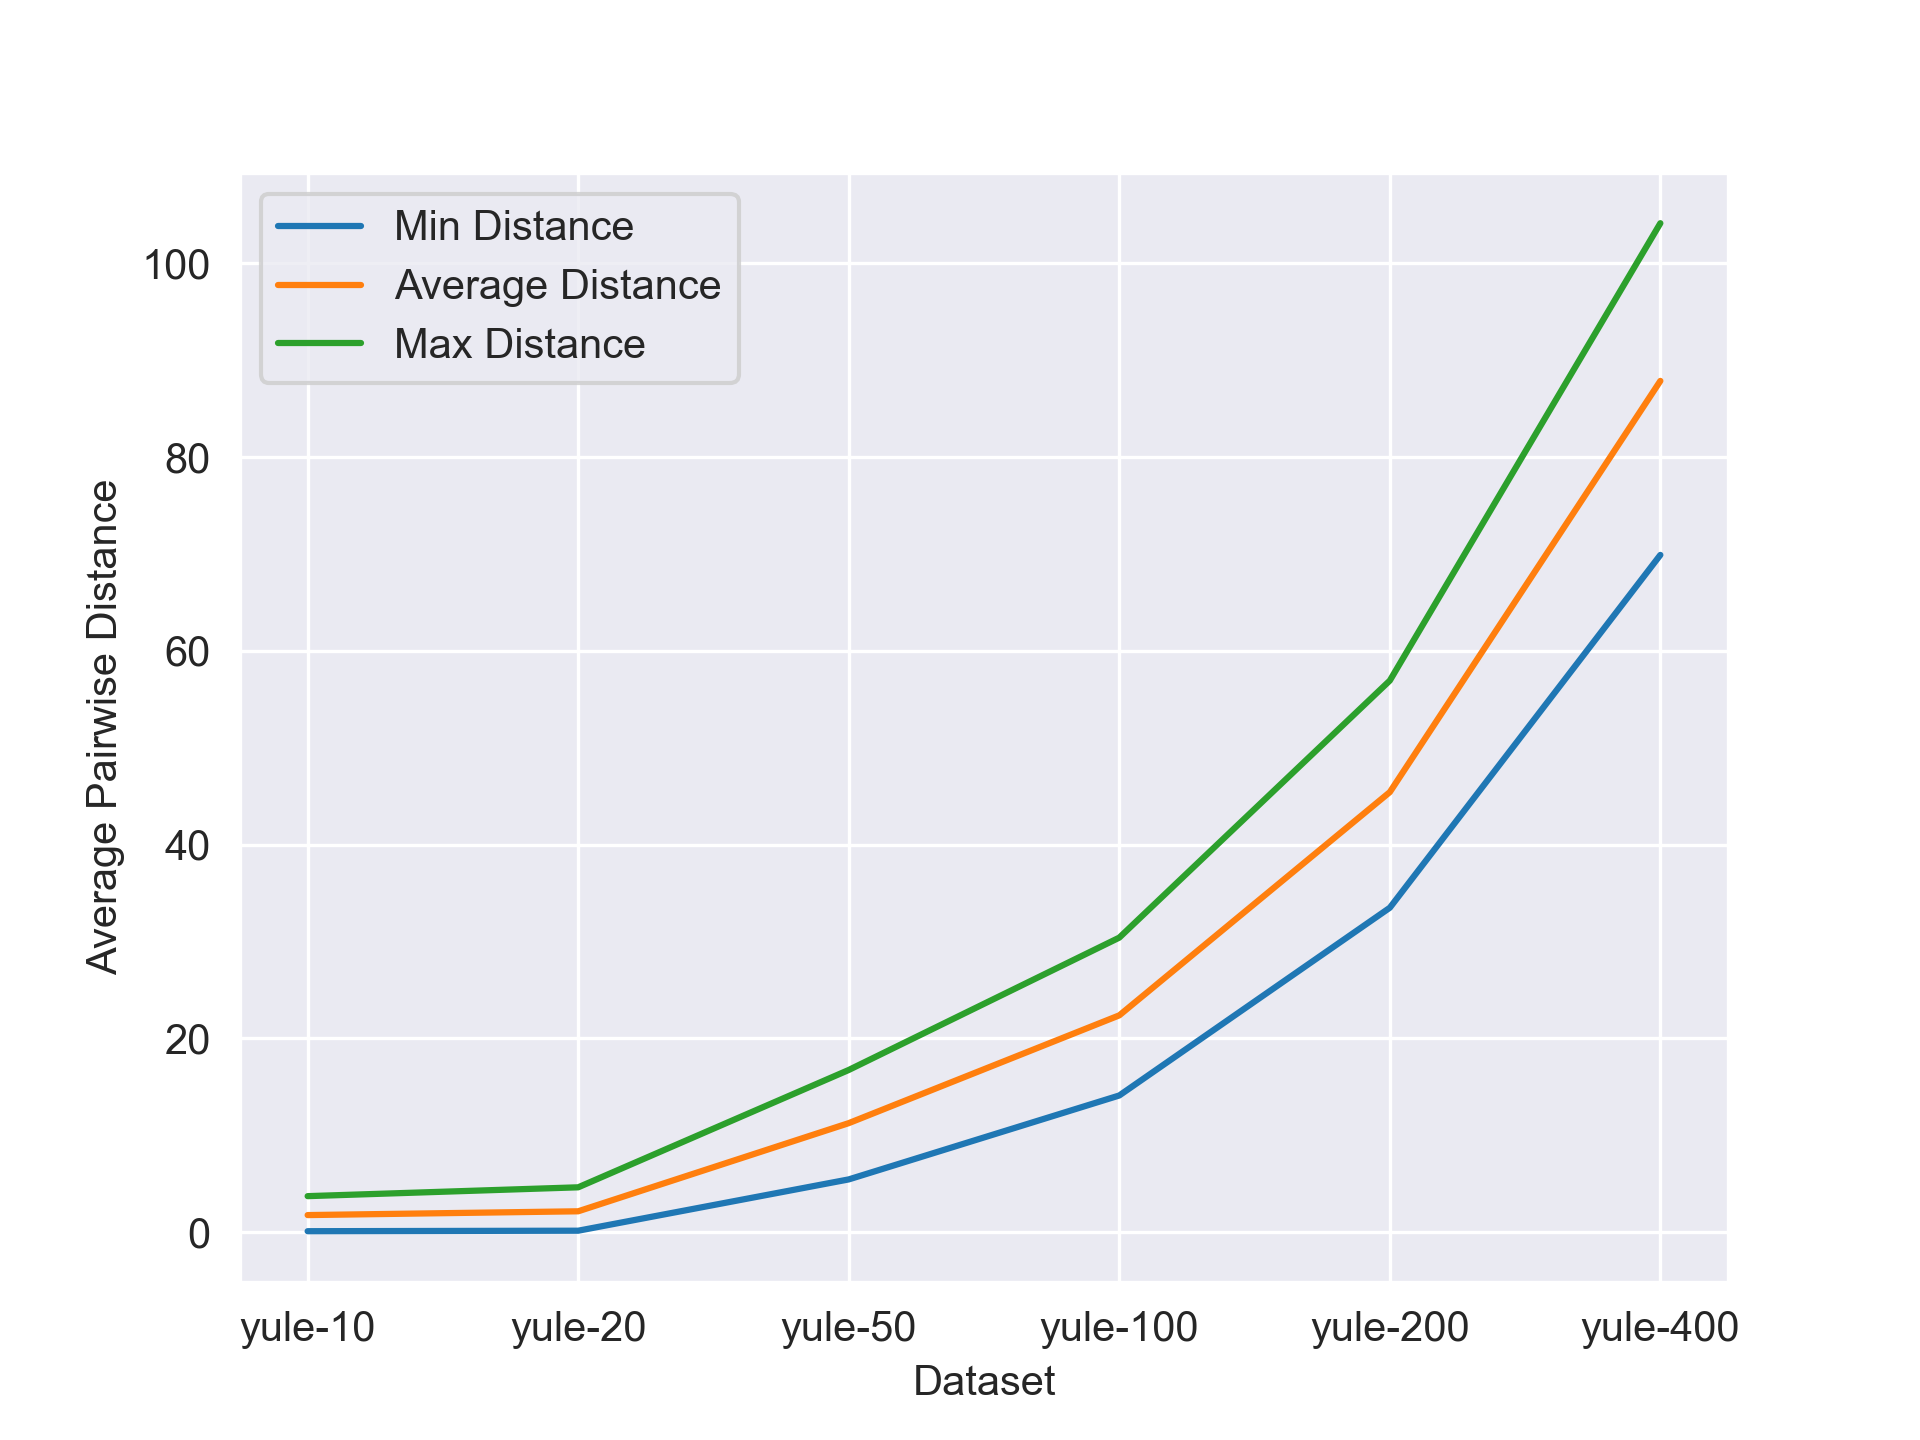
\includegraphics[width=\textwidth]{figures/curse_distance.png}
        \caption{The average pairwise Robinson–Foulds distance between the MCMC trees of the synthetic Yule datasets. The distances increase with the number of taxa.}

		\label{fig:curse1}
    \end{minipage}
    \hfill
    \begin{minipage}[t]{0.45\textwidth}
        \centering
        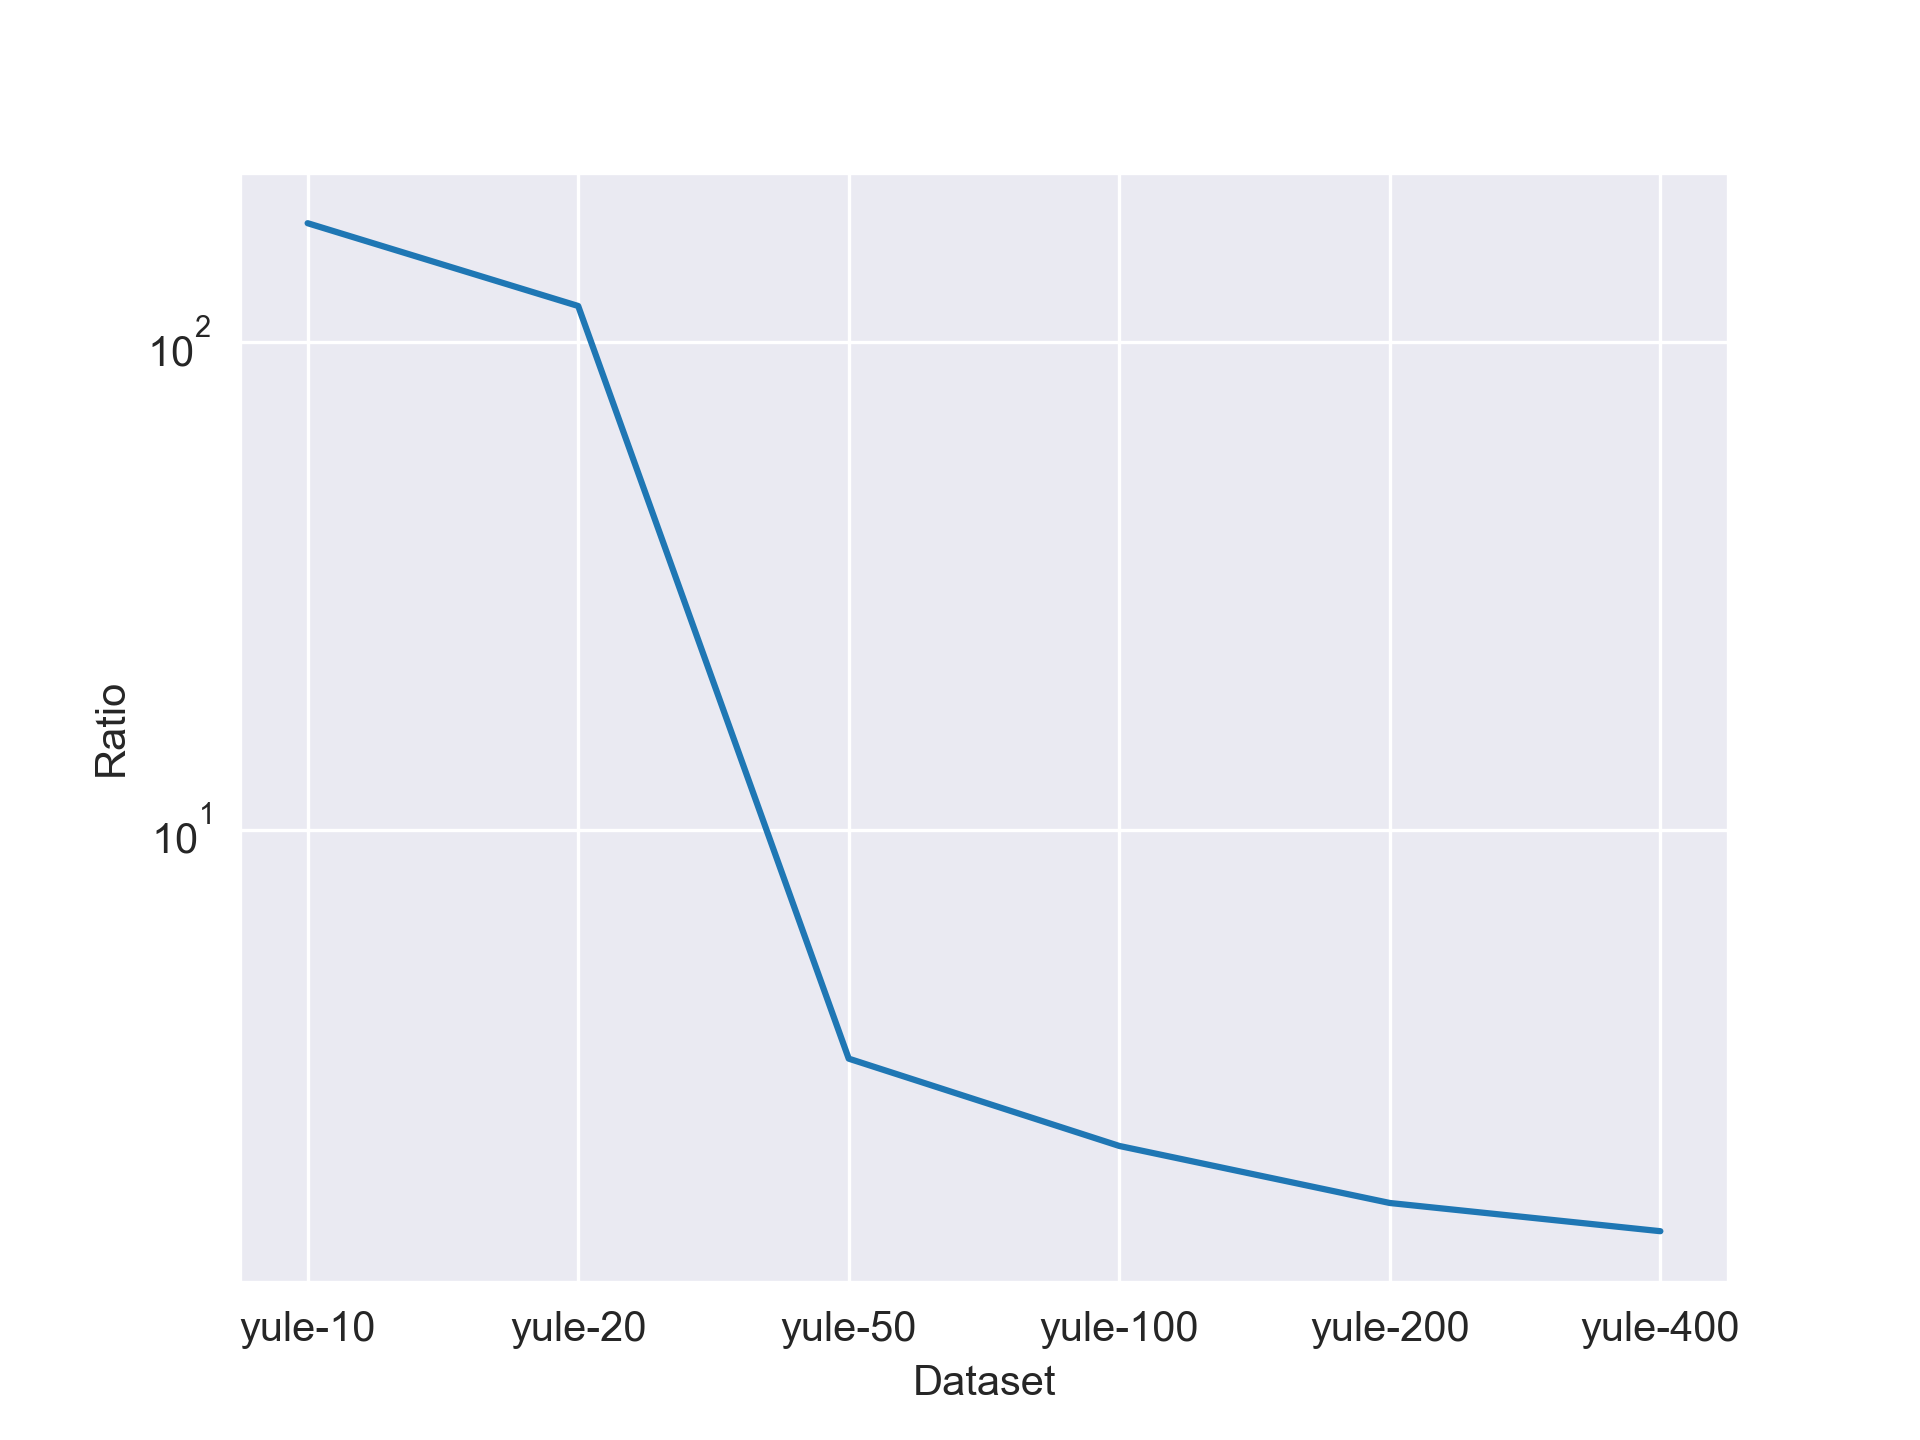
\includegraphics[width=\textwidth]{figures/curse_ratio.png}
        \caption{The average ratio of the minimum to maximum pairwise Robinson–Foulds distance between the MCMC trees of the synthetic Yule datasets. The ratios decrease with the number of taxa.}

		\label{fig:curse2}
    \end{minipage}
\end{figure}

\subsection*{Tree dirichlet distribution}

\subsection*{Datasets}

\nolinenumbers

\bibliography{refs}

\end{document}

